\subsection{Content Analysis in Advertising}

Automatic content analysis can be found useful in many different settings, but the two of the most dominating areas are advertising and improvement of user experience. The context of this project is to improve advertising, which makes advertising our domain.

Advertising is the main income of most online companies that provide free services. The alternative to advertising is to charge users, which means that they have to pay a fee in order to use the services. The World Wide Web is very competitive and most users expect everything on the Internet to be free. For this reason the most common approach is to provide the services for free, and earn money on advertising instead. 

There are mainly four different roles within online advertising \cite{onlineadhowdoesitworks}. These roles may overlap so that the same person or company can possess than one role. 
\begin{enumerate}
\item The advertisers, also called marketers, are people or a companies that have advertisements they want to display on webpages. The advertisers are willing to pay more for advertisements if the webpages are frequently visited or if the advertisements are displayed to users with a higher potential of buying the products. 
\item The brokers, usually a third-party advertising company, manages the selection of advertisements and the placements of these. These companies collect information about the Internet users so that the advertisements are directed towards potential customers. 
\item The publishers are people or companies in charge of a webpage with advertisement spaces. They sell the advertisement spaces, but the brokers are the ones responsible for choosing which advertisements to show.
\item Ad-Tech players are companies between the advertisers and the publishers. These companies get paid to provide information to optimize the advertising, which is profitable for the other roles within online advertising. 

\end{enumerate}
All roles within online advertising have a higher probability of earning money if the advertisements are chosen based on the interests of the users. 
This is called \emph{Interest-Based Advertising (IBA)} or \emph{Online Behavioral Advertising (OBA)}, where the advertisements are chosen depending on the user's interests or browsing history. Information about browsing performed by users are collected at all times so that advertisements displayed are more likely to be relevant for each user (see figure \ref{fig:interestbasedadvertising} \cite{onlineadwhatisit}).

\begin{figure}[h]
\centering
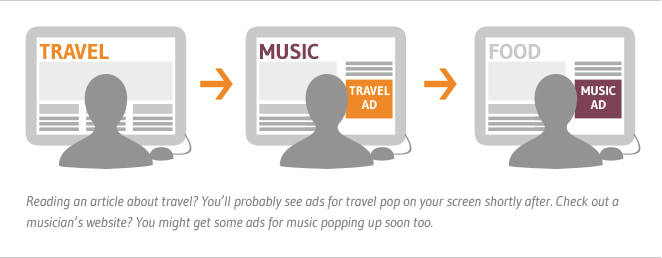
\includegraphics[width=\textwidth]{Chapters/Background/Interest_based_advertising}
\caption[Retargeting within Interest-based Advertising]{Illustration of retargeting which is a advertising technique within Interest-based Advertising (IBA).}
\label{fig:interestbasedadvertising}
\end{figure}
\begin{comment}
All roles within the advertising can earn more money if the advertisements
are pleased if the advertisements are shown to users more likely to buy the products. 
There are three main approaches of online advertising as well. \cite{onlineadwhatisit}
\end{comment}

There are two different approaches of performing online advertising. % TODO INSERT REFERENCE
\begin{enumerate}
\item \emph{Display Advertising} is a method where the advertiser pays for each display of the advertisement on a webpage. There are different ways of computing the cost of display advertising, but the most common is \emph{Cost-Per-Mille} (CPM) or \emph{cost-per-thousand impressions}. CPM is a metric where the advertiser pays for showing the advertisement to thousand viewers \cite{costperthousandimpressions}, and popular pages have a higher CPM than unpopular pages. 
\item \emph{Affiliate marketing} is based on the success of the advertisement. One of the most common approaches within this affiliate marketing is  \emph{Performance-based advertising} where the price of the advertisement is based on the interaction with the user, i.e., how successful the advertisement is 
%interaction with the user determine the price of the advertisement. 
%of interactive advertising where the price of the advertisements depends on the performance of the advertisement. 
%This means that the price of an advertisement is based on the interaction of the user 
\cite{performancebasedad}. There are different ways of measuring the advertisement's success. The most common ones are:
%is method is usually split into two common measurements: 
\begin{itemize}
\item \emph{Cost-Per-Click} (CPC) where the advertiser pays per click on the advertisement \cite{costperclick}.
\item \emph{Cost-Per-Action} (CPA) where the price of the advertisement is also based on the probability of a completed transaction \cite{costperaction}.
%clicks your ad will go on to complete your desired action, whether it’s making a purchase or filling out a form to become a lead. Cost per action takes into account the number of ad clicks you need b
\end{itemize}
%how often it is viewed on a webpage, how often the users click on the advertisement and how often it leads to an actual sale \cite{performancebasedad}.
\end{enumerate}


%ones are Pay-Per-Click (PPC) \cite{wiki:ppc} and Cost-Per-Mille (CPM) \cite{wiki:ppc}. PPC is an approach where the advertiser pays per click on the advertisements, while CPM means that the advertiser pays for showing the advertisement to thousand viewers. 
All these approaches are more valuable for all roles in the advertising process if the advertisements are shown to people that are interested in the products and more likely to buy the product. Thus, our motivation is to improve advertising by creating a content classifier that categorizes text into suitable categories which is a great help when building up user profiles.

